%\documentclass[0-main.tex]{subfiles}
%\begin{document}

\section{Experiments}\label{sec:exp}
We evaluate \hirl on two standard RL benchmarks and in deformable cutting and tensioning on the da Vinci surgical robot.

\begin{figure}[t]
\centering
 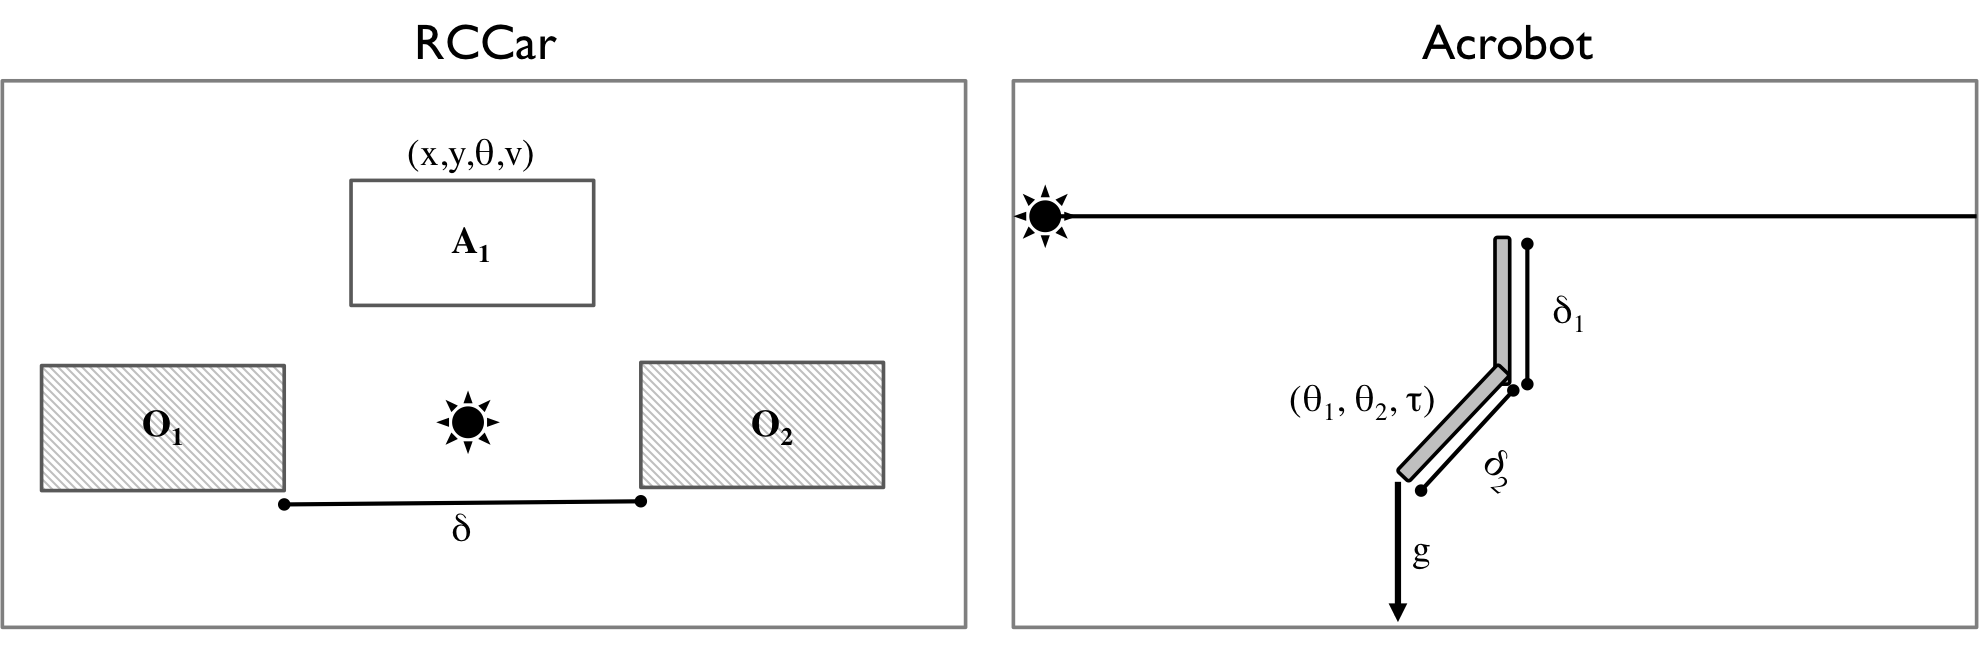
\includegraphics[width=\columnwidth]{figures/domains.png}
 \caption{(A) Simulated control task with a car with noisy non-holonomic dynamics. The car ($A_1$) is controlled by accelerating and turning in discrete increments. The task is to park the car between two obstacles. \label{domains}}
\end{figure}

\begin{figure}[t]
\centering
 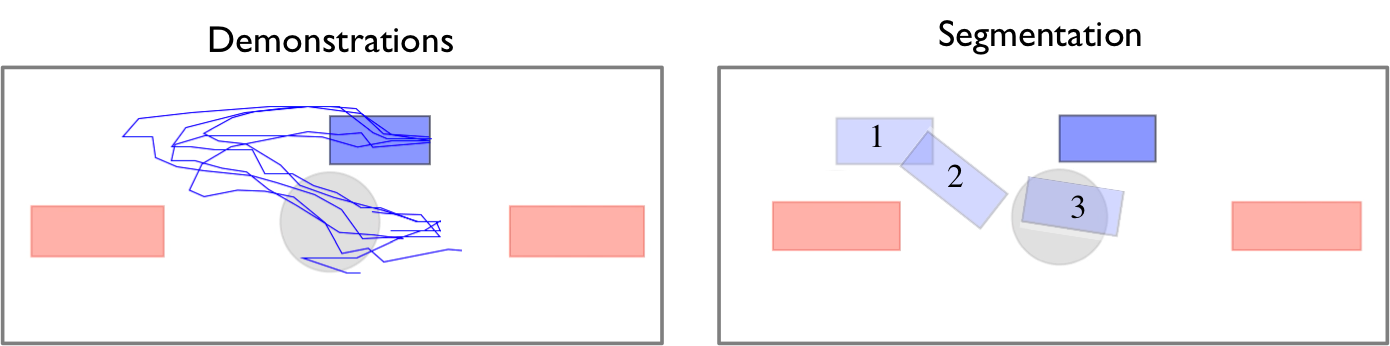
\includegraphics[width=\columnwidth]{exp/rc-car-segmentation.png}
 \caption{(Left) the 5 demonstration trajectories for the parallel parking task, and (Right) the sub-goals learned by \hirl. There are two intermediate goals corresponding to positioning the car and orienting the car correctly before reversing. \label{exp:rcsegmentation}}
\end{figure}

\subsection{Fully Observed Parallel Parking}\label{exp:pp}
We constructed a parallel parking scenario for a robot car with non-holonomic dynamics and two obstacles (Figure \ref{domains}a). 
The car can accelerate or decelerate in discrete $\pm 0.1$ meters per second increments (and reverse), and change its heading by $5^\circ$ degree increments.
The car's speed ($\|\dot{x}\|+\|\dot{y}\|$) and heading ($\theta$) are inputs to a bicycle steering model which computes the next state.
The car observe its x position, y position, orientation, and speed in a global coordinate frame.
The robot's dynamics are noisy and with probability 0.1 will randomly add or subtract $2.5^\circ$ degrees to the steering angle.
If the robot parks between the obstacles, i.e., 0 speed within a $15^\circ$ tolerance and a positional tolerance of $5$ meters, the task is a success and the robot receives a reward of $1$. 
If the robot collides with one of the obstacle or does not park in 200 timesteps the episode ends with a reward of $0$.

We call this domain Parallel Parking with Full Observation (PP-FO). We consider the following approaches:

\vspace{0.25em}\noindent \textbf{RL (Q-Learning): } The baseline approach is modeling the entire problem as an MDP with the sparse delayed reward. We apply Q-Learning to learn a policy for this problem with a radial basis function representation for the Q function with number of bases and bandwidth $k=5, \sigma=0.1$ respectively. The radial basis function hyper-parameters were tuned manually to achieve the fastest convergence in the experimental task. 

\vspace{0.25em}\noindent \textbf{Behavioral Cloning (SVM): } We generated $N$ demonstrations using an RRT motion planner (assuming deterministic dynamics). The next baseline is to directly learn a policy from the generated plans using behavioral cloning. We use a L1 hinge-loss SVM with L2 regularization $\alpha=5e-3$ to predict the action from the state. The hyper-parameters were tuned manually using cross-validation by holding out trajectories.

\vspace{0.25em}\noindent \textbf{Single-Step IRL (MaxEnt-IRL): } We generated $N$ demonstrations using an RRT motion planner (assuming deterministic dynamics). We use the collected demonstrations and infer a quadratic reward function using MaxEnt-IRL (both using estimated dynamics and ground truth dynamics). The learned reward function is optimized using Q-learning with a radial basis function representation with the same hyper-parameters as the RL approach. 

\vspace{0.25em}\noindent \textbf{\hirl: } Finally, we apply \hirl to the $N$ demonstrations, learn segmentation, and quadratic rewards (Figure~\ref{exp:rcsegmentation}).
We apply \hirl with a DP-GMM based segmentation step with no kernel transformation (as described in Section \ref{segm}).
For the local IRL approach, we consider three approaches: MaxEnt with ground truth dynamics, MaxEnt with locally estimated dynamics, Model-Free. 
The learned reward functions and transition regions are used in the policy learning phase with Q-learning with a radial basis function representation with the same hyper-parameters as the RL approach.

\vspace{0.5em}

\begin{figure}[t]
\centering
 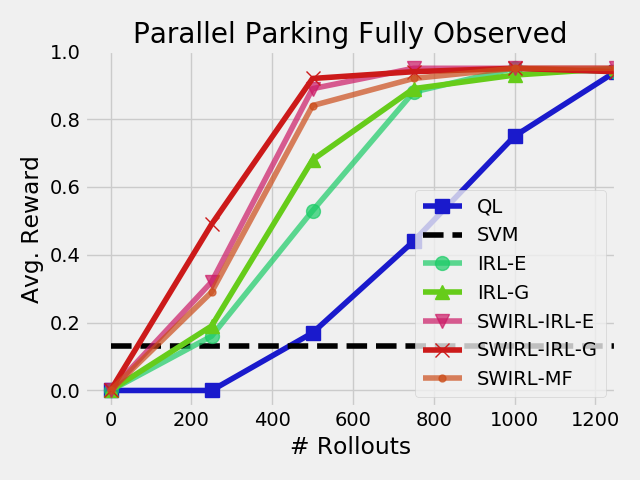
\includegraphics[width=0.8\columnwidth]{new-exp/pp-fo.png}
 \caption{For a fixed number of demonstrations $5$, we vary the number of rollouts and measure the average reward at each rollout. (QL) denotes Q-learning, (SVM) denotes a baseline of behavioral cloning with a SVM policy representation, (IRL-E) denotes MaxEnt-IRL with estimated dynamics, (IRL-G) denotes MaxEnt-IRL with ground truth dynamics, (SWIRL-E) denotes SWIRL with local MaxEnt-IRL and estimated dynamics, (SWIRL-G) denotes SWIRL with local MaxEnt-IRL and ground truth dynamics, and (SWIRL-MF) denotes the model-free version of SWIRL. SWIRL achieves the same reward as QL with 15\% of the rollouts, and the same reward as IRL with 66\% of the rollouts. \label{exp:pp-fo1}}
\end{figure}

\subsubsection{Fixed Demonstrations, Vary Rollouts}
In the first experiment, we fix number of initial demonstrations $N=5$, and vary the number of rollouts (Figure \ref{exp:pp-fo1}).
The basline line Q-Learning approach (QL) is very slow, because it relies on random exploration to achieve the goal at least once before it can start estimating the value of states and actions.
However, given enough exploration (1250 rollouts), Q-Learning converges to a solution with a 95\% success rate.
In this problem, there will always be some failure cases to the noise in the system.
We collect 5 demonstrations and directly learn a policy with an SVM.
This policy has a very poor success rate of 13\%.
Q-Learning and the SVM define two extremes, no demonstrations and no rollouts, respectively.

Next, we consider combinations of rollouts and demonstrations.
We apply MaxEnt-IRL to the 5 demonstrations and learn reward functions.
Since the MaxEnt-IRL inference procedure requires a dynamics model, we consider two variants: (1) estimate the dynamics from the demonstrations, and (2) use the known dynamics model of the car directly.
We found that both IRL methods surpassed the SVM policy after only 250 rollouts, and attained the same final reward as Q-Learning in 250 less rollouts.
Surprisingly, we found that there was little difference between using the estimated dynamics model and the ground truth model.

Finally, we considered three variants of \hirl. (SWIRL-E) is SWIRL with local MaxEnt-IRL and estimated dynamics, (SWIRL-G) is SWIRL with local MaxEnt-IRL and ground truth dynamics, and (SWIRL-MF) denotes the model-free version of SWIRL.
SWIRL achieves the same reward as QL with 15\% of the rollouts, and the same reward as IRL with 66\% of the rollouts.
\hirl learns three segments for this task (Figure~\ref{exp:rcsegmentation}), and places quadratic rewards that guide the car to each of these segments.
There are two intermediate goals corresponding to positioning the car and orienting the car correctly before reversing.
With a single quadratic reward (as in IRL), the car has to learn to make a sequence of actions that move away from the goal (pulling up). In the segmented problem, the car can always move monotonically towards each of the goals.


\begin{figure}[t]
\centering
 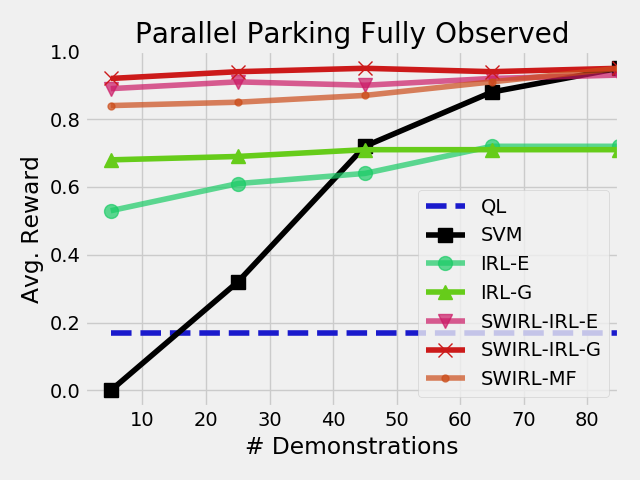
\includegraphics[width=0.8\columnwidth]{new-exp/pp-fo2.png}
 \caption{For a number of rollouts $500$, we vary the number of demonstration trajectories given to each technique. (QL) denotes Q-learning, (SVM) denotes a baseline of behavioral cloning with a SVM policy representation, (IRL-E) denotes MaxEnt-IRL with estimated dynamics, (IRL-G) denotes MaxEnt-IRL with ground truth dynamics, (SWIRL-E) denotes SWIRL with local MaxEnt-IRL and estimated dynamics, (SWIRL-G) denotes SWIRL with local MaxEnt-IRL and ground truth dynamics, and (SWIRL-MF) denotes the model-free version of SWIRL. SWIRL is less senstive to the number of demonstrations observed than the SVM. With only 5 demonstrations, SWIRL is within 10\% of its reward if it observed 100 demonstrations. \label{exp:pp-fo2}}
\end{figure}

\subsubsection{Fixed Rollouts, Vary Demonstrations}
Next, we fix the number of rollouts to $500$, and vary the number of demonstration trajectories each approach observes.
The basline line Q-Learning approach (QL) takes no demonstrations and has a success rate of 17\% after 500 rollouts.
The behavioral cloning approach (SVM) is sensitive to the number of demonstrations it observes. 
For 5 demonstrations, it acheives a success rate of only 13\%.
But if it observes 100 demonstrations it can achieve nearly the maximum 95\% success rate.

On the other hand, the IRL approaches and SWIRL are comparatively less sensitive--where they perform nearly as well with a small number of demonstrations as they do with a larger dataset.
With only 5 demonstrations, SWIRL is within 10\% of its reward if it observed 100 demonstrations.
In this task the policy is more complex than the reward function, which is just a quadratic.
It potentially requires much less data to estimate a quadratic function.

The SVM approach does have the advantage that it doesn't require any further exploration.
However, SWIRL and the SVM approach are not mutually exclusive. 
As we show in our physical experiments, we can initialize Q-learning with a behavioral cloning policy. 
The combination of the two approaches allows us to take advantage of a small number of demonstrations and learn to refine the initial policy through exploration.


\begin{figure}[t]
\centering
 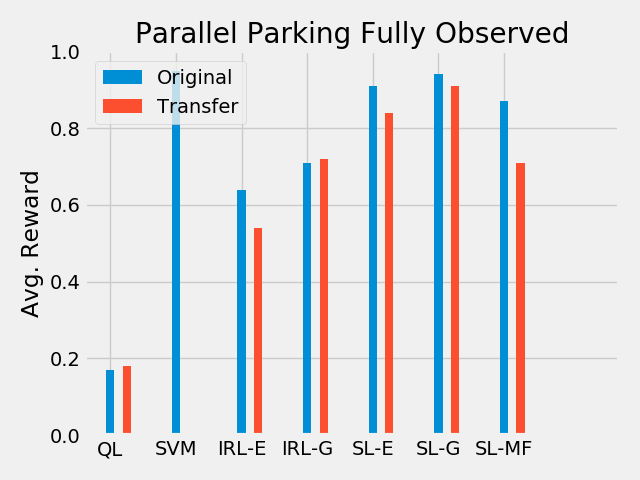
\includegraphics[width=0.8\columnwidth]{new-exp/pp-fo3.png}
 \caption{For $500$ rollouts  and $100$ demonstrations, we measure the robustness of the approaches to changes in the execution dynamics. (QL) denotes Q-learning, (SVM) denotes a baseline of behavioral cloning with a SVM policy representation, (IRL-E) denotes MaxEnt-IRL with estimated dynamics, (IRL-G) denotes MaxEnt-IRL with ground truth dynamics, (SL-E) denotes SWIRL with local MaxEnt-IRL and estimated dynamics, (SL-G) denotes SWIRL with local MaxEnt-IRL and ground truth dynamics, and (SL-MF) denotes the model-free version of SWIRL. While the SVM is 95\% successful on the original domain, its success does not transfer to the perturbed setting. On the other hand, SWIRL learns rewards and segments that transfer to the new dynamics since they are state-space goals. \label{exp:pp-fo3}}
\end{figure}

\subsubsection{Varying Task Parameters}
We also explored how well the approaches handle transfer if the dynamics change between demonstration and execution.
We collect demonstrations $N=100$ on the original task, and then used the learned rewards or policies on a perturbed task.
In the perturbed task, the system dynamics are coupled in a way that turining right causes the car to accelerate forward by $0.05$ meters per second.
So in the perturbed task the car must learn to adjust to this acceleration during the reversing phase.
In the new domain, each approach is allowed $500$ rollouts. 
We report the results (Figure \ref{exp:pp-fo3}).

The success rate of the policy learned with Q-Learning is more or less constant between the two domains.
This is because Q-learning does not use any information from the original domain.
The SVM behavioral cloning policy has a drastic change.
On the original domain with a 100 demonstrations it acheives a 95\% success rate, however, on the perturbed domain it is never successful.
This is because the SVM learned a policy that causes it to crash into one of the obstacles in the perturbed environment.

The IRL techniques are more robust during the transfer.
This is because the rewards learned are quadratic functions of the state and do not encode anything specific about the dynamics.
Similarly, in SWIRL, the rewards and transition regions are invariant to the dynamics in this transfer problem.
For SWIRL-E and SWIRL-G, there is only a drop of 5\% in the success rate.
On the other hand, the model-free version of SWIRL reports a larger drop of 16\%.
This is because the model-free version is not a true IRL algorithm and may enocde some aspects of the dynamics in the learned reward function.

Coincidentally, this experiment also shows us how to construct a failure mode for \hirl.
If the perturbation in the task is such that it ``invalidates'' a transition region, e.g., a new obstacle, then \hirl may not be able to learn to complete the task.
However, the transition regions give us a formalism to detecting such problems during learning as we can keep track of which regions are possible to reach.


\begin{figure}[t]
\centering
 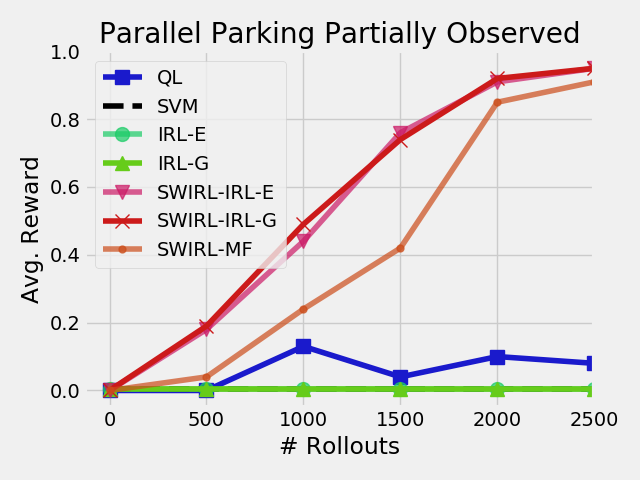
\includegraphics[width=0.8\columnwidth]{new-exp/pp-po.png}
 \caption{We hid the velocity state from the robot, so the robot only sees $(x,y,\theta)$. For a fixed number of demonstrations $5$, we vary the number of rollouts and measure the average reward at each rollout. (QL) denotes Q-learning, (SVM) denotes a baseline of behavioral cloning with a SVM policy representation, (IRL-E) denotes MaxEnt-IRL with estimated dynamics, (IRL-G) denotes MaxEnt-IRL with ground truth dynamics, (SWIRL-E) denotes SWIRL with local MaxEnt-IRL and estimated dynamics, (SWIRL-G) denotes SWIRL with local MaxEnt-IRL and ground truth dynamics, and (SWIRL-MF) denotes the model-free version of SWIRL. SWIRL converges will the other approaches fail to reach a reliable success rate \label{exp:pp-po}}
\end{figure}


\subsubsection{Partially Observed Parallel Parking}
Next, we made the Parallel Parking domain more difficult to illustrate the connection between segmentation and memory in RL. 
We hid the velocity state from the robot, so the car only sees $(x,y,\theta)$. 
As before, if the car collides with one of the obstacle or does not park in 200 timesteps the episode ends.
We call this domain Parallel Parking with Partial Observation (PP-PO).

This form of partial observation creates an interesting challenge.
There is no longer a stationary policy that can achieve the reward.
During the reversing phase of parallel parking, the car does not know that it is currently reversing.
So there is ambiguity in that state whether to pull up or reverse.
We will see that segmentation can help disambiguate the action in this state.

As before, we generated 5 demonstrations using an RRT motion planner (assuming deterministic dynamics) and applied each of the approaches.
The techniques that model this problem with a single MDP all fail to converge.
The Q-Learning approach achieves some non-zero rewards by chance.
The learned segments in \hirl help disambiguate dependence on history, since the segment indicator tells the car which stage of the task is currently active (pulling up or reversing)
After 250000 time-steps, the policy learned with model-based \hirl has a 95\% success rate in comparison to a <10\% success rate for the baseline RL, 0\% for MaxEnt-IRL, and 0\% for the SVM.


\begin{figure*}[t]
\centering
 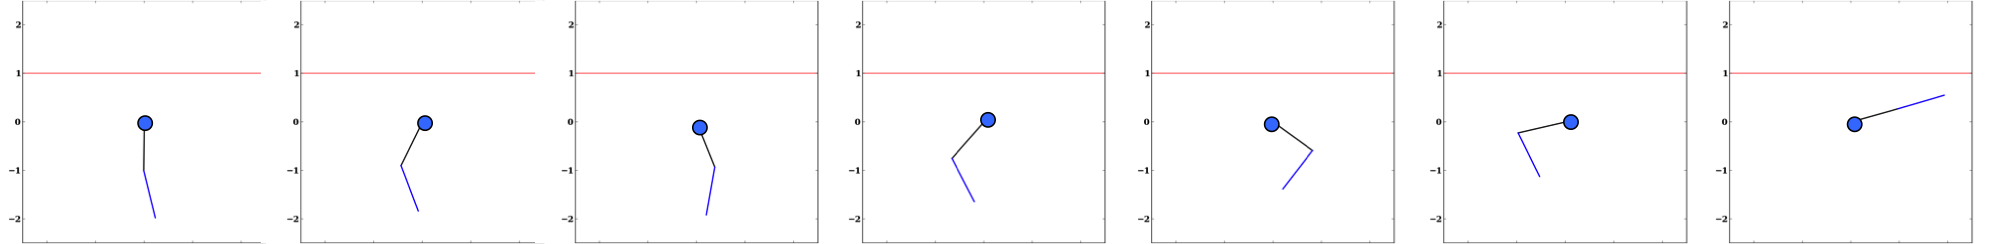
\includegraphics[width=0.8\textwidth]{exp/segmentation-acrobot-segments.png}
 \caption{We plot the centroids of the learned segments in \hirl to visualize how \hirl is partitioning the task. Qualitatively, \hirl constructs evenly-spaced way points along the swing up trajectory.  \label{acr-segments}}
\end{figure*}


\subsection{Acrobot}\label{exp:acrobot}
This domain consists of an under-actuated two-link pendulum with gravity and with torque controls on the joint (Figure \ref{domains}b). 
There are 4 discrete actions that correspond to clockwise and counter-clockwise torques on each of the links. 
The robot observes the angle $\theta_1, \theta_2$ and angular velocity $\omega_1, \omega_2$ at each of the links.
The dynamics are noisy where a small amount of random noise is added to each torque applied to the pendulum. 
The robot has 1000 timesteps to raise the arm above horizontal ($y=1$ in the image). If the task is successful and the robot receives a reward of $1$. 
The expected reward is equivalent to the probability that the current policy will successfully raise the arm above horizontal.

This task is interesting because the underlying system is non-linear. 
Many IRL algorithm require dynamics to estimate the reward and non-linearities may not have closed form solutions.
In this experiment, we show that linearizing the dynamics based on the demonstrations is a reasonable idea in \hirl.
Since we are fitting a piecewise reward, the system need only be locally linear.
This coulped with a kernel transformation empirically gives segmented rewards that improve convergence.

We considered the following baselines:

\vspace{0.25em}\noindent \textbf{RL (Q-Learning): } The baseline approach is modeling the entire problem as an MDP with the sparse delayed reward. We apply Q-Learning to learn a policy for this problem with a radial basis function representation for the Q function with number of bases and bandwidth $k=25, \sigma=0.25$ respectively. The radial basis function hyper-parameters were tuned manually to achieve the fastest convergence in the experimental task. 

\vspace{0.25em}\noindent \textbf{Behavioral Cloning (Kernel SVM): } We generated $N$ demonstrations using the Q-Learning baseline (i.e., run to convergence and sample from the learned policy). We use an RBF kernel SVM $\sigma=1e-5$  with L2 regularization $\alpha=5e-3$ to predict the action from the state. The hyper-parameters were tuned manually using cross-validation by holding out trajectories.

\vspace{0.25em}\noindent \textbf{Single-Step IRL (MaxEnt-IRL): } We generated $N$ demonstrations using the Q-Learning baseline (i.e., run to convergence and sample from the learned policy). We use the collected demonstrations and infer a quadratic reward function using MaxEnt-IRL. In the acrobot, we only use estimated dynamics because the underlying system is non-linear. The estimated dynamics are a linearization. The learned reward function is optimized using Q-learning with a radial basis function representation with the same hyper-parameters as the RL approach. 

\vspace{0.25em}\noindent \textbf{\hirl: } Finally, we apply \hirl to the $N$ demonstrations, learn segmentation, and quadratic rewards (Figure~\ref{exp:rcsegmentation}).
We apply \hirl with a DP-GMM based segmentation step with a kernel transformation $\sigma = 0.1$ (as described in Section \ref{segm}).
For the local IRL approach, we consider two approaches: MaxEnt with locally estimated dynamics, Model-Free. 
The learned reward functions and transition regions are used in the policy learning phase with Q-learning with a radial basis function representation with the same hyper-parameters as the RL approach.


\begin{figure}[t]
\centering
 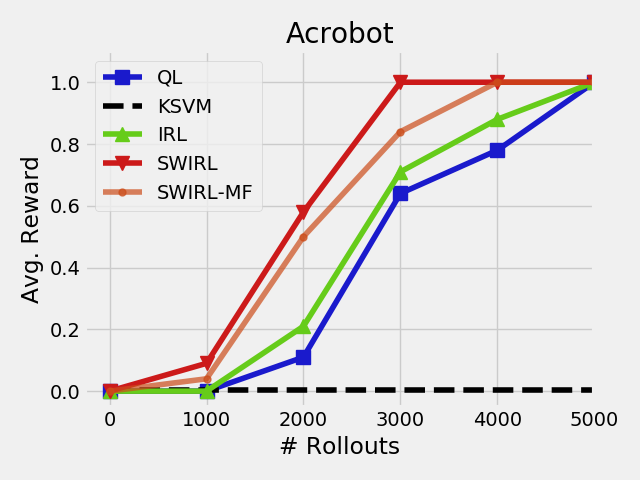
\includegraphics[width=0.8\columnwidth]{new-exp/acr.png}
 \caption{For a fixed number of demonstrations $5$, we vary the number of rollouts and measure the average reward at each rollout. (QL) denotes Q-learning, (KSVM) denotes a baseline of behavioral cloning with a Kernel SVM policy representation, (IRL) denotes MaxEnt-IRL using linearized dynamics learned from the demonstrations, (SWIRL) denotes SWIRL with local MaxEnt-IRL and estimated linear dynamics, and (SWIRL-MF) denotes the model-free version of SWIRL. SWIRL converges with 2000 fewer rollouts than Q-learning and IRL. \label{exp:acr}}
\end{figure}


\subsubsection{Fixed Demonstrations, Vary Rollouts}
We generated $N=15$ demonstrations for the Acrobot task and compared the different approaches (Figure \ref{exp:acr}). 
The baseline behavioral cloning policy with a kernel svm failed to succeed.
Q-learning required 5000 rollouts to acheive a policy that was successful 100\% of the time.
IRL did not converge significantly faster than Q-Learning.
This is because it models the reward function as a single quadratic, but there are multiple steps required to swing the pendulum up.
The single quadratic potentially misleads learner in early episodes.

Finally, we see that SWIRL converges with 2000 fewer rollouts than Q-learning and IRL.
The model-free method converges with 1000 more rollouts.
This experiment suggests that \hirl is applicable to certain types of non-linear systems.
We defer a more formal study of this problem to future work. 


\begin{figure}[t]
\centering
 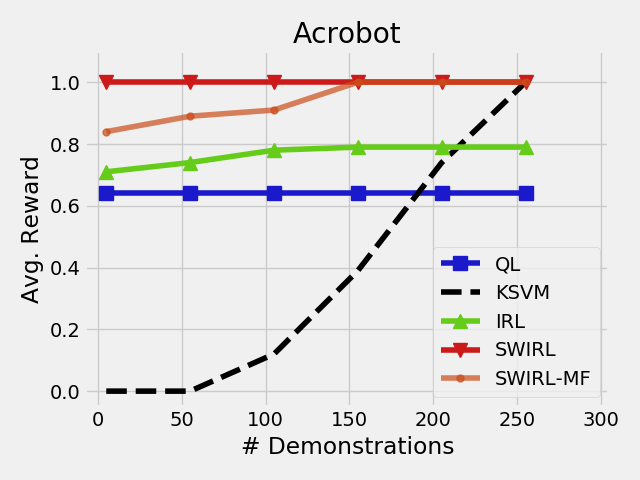
\includegraphics[width=0.8\columnwidth]{new-exp/acr2.png}
 \caption{For a number of rollouts $3000$, we vary the number of demonstration trajectories given to each technique. QL) denotes Q-learning, (KSVM) denotes a baseline of behavioral cloning with a Kernel SVM policy representation, (IRL) denotes MaxEnt-IRL using linearized dynamics learned from the demonstrations, (SWIRL) denotes SWIRL with local MaxEnt-IRL and estimated linear dynamics, and (SWIRL-MF) denotes the model-free version of SWIRL. SWIRL is less senstive to the number of demonstrations observed than the SVM. With only 15 demonstrations, SWIRL is able to achieve the maximum reward. In comparison, the SVM requires 250 demonstrations. \label{exp:acr2}}
\end{figure}


\subsubsection{Vary Demonstrations, Fixed Rollouts}
Next, we fix the number of rollouts to $3000$, and vary the number of demonstration trajectories each approach observes (Figure \ref{exp:acr2}).
This task is substantially harder to learn than the parallel parking task.
More demonstration data is required to learn the segments, rewards, and policies.
The basline line Q-Learning approach (QL) takes no demonstrations and has a success rate of 58\% after 3000 rollouts.
As before, the behavioral cloning approach (KSVM) is sensitive to the number of demonstrations it observes. 
For 50 demonstrations, it acheives a success rate of 0\%.
It requires 250 demonstrations to have a 100\% success rate.
Again, the IRL approaches and SWIRL are less sensitive--where they perform nearly as well with a small number of demonstrations as they do with a larger dataset.
With only 15 demonstrations, SWIRL is able to achieve the maximum reward.


\begin{figure}[t]
\centering
 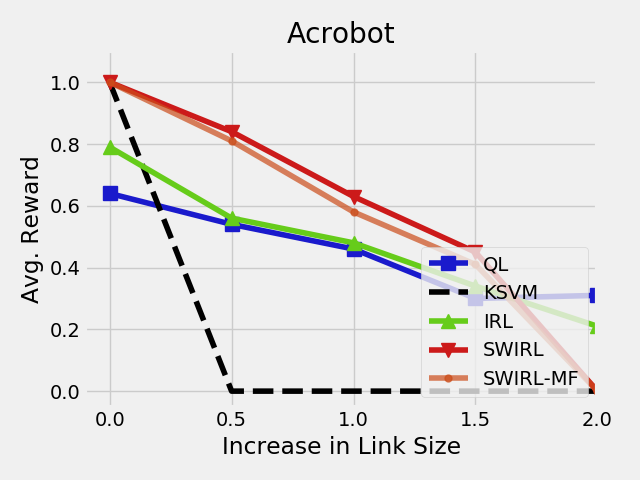
\includegraphics[width=0.8\columnwidth]{new-exp/acr3.png}
 \caption{For a number of rollouts $3000$ and $250$ demonstrations, we measure the transfer as a function of varying the link size. (QL) denotes Q-learning, (KSVM) denotes a baseline of behavioral cloning with a Kernel SVM policy representation, (IRL) denotes MaxEnt-IRL using linearized dynamics learned from the demonstrations, (SWIRL) denotes SWIRL with local MaxEnt-IRL and estimated linear dynamics, and (SWIRL-MF) denotes the model-free version of SWIRL. The KSVM policy fails as soon the link size is changed. SWIRL is robust until the change becomes very large.  \label{exp:acr3}}
\end{figure}


\subsubsection{Vary Task Parameters}
As in the parallel parking scenario, we evaluate how the different approaches handle transfer if the dynamics change between demonstration and execution.
With $N=250$ demonstrations, we learn the rewards, policies, and segments on the standard pendulum, and then during learning, we vary the size of the second link in the pendulum.
We plot the success rate (after a fixed 3000 rollouts) as a function of the increasing link size (Figure \ref{exp:acr3}).

As the link size increases the even the basline Q-learning becomes less successful. This is because the system becomes more unstable and it is harder to learn a policy.
The behavioral cloning SVM policy immediately fails as the link size is increased.
IRL is more robust but does not offer much of an advantage in this problem.
\hirl is robust until the change in the link size becomes large.
This is because for the larger link size, \hirl might require different segments (or one of the learned segments in unreachable).



\begin{figure}[t]
\centering
    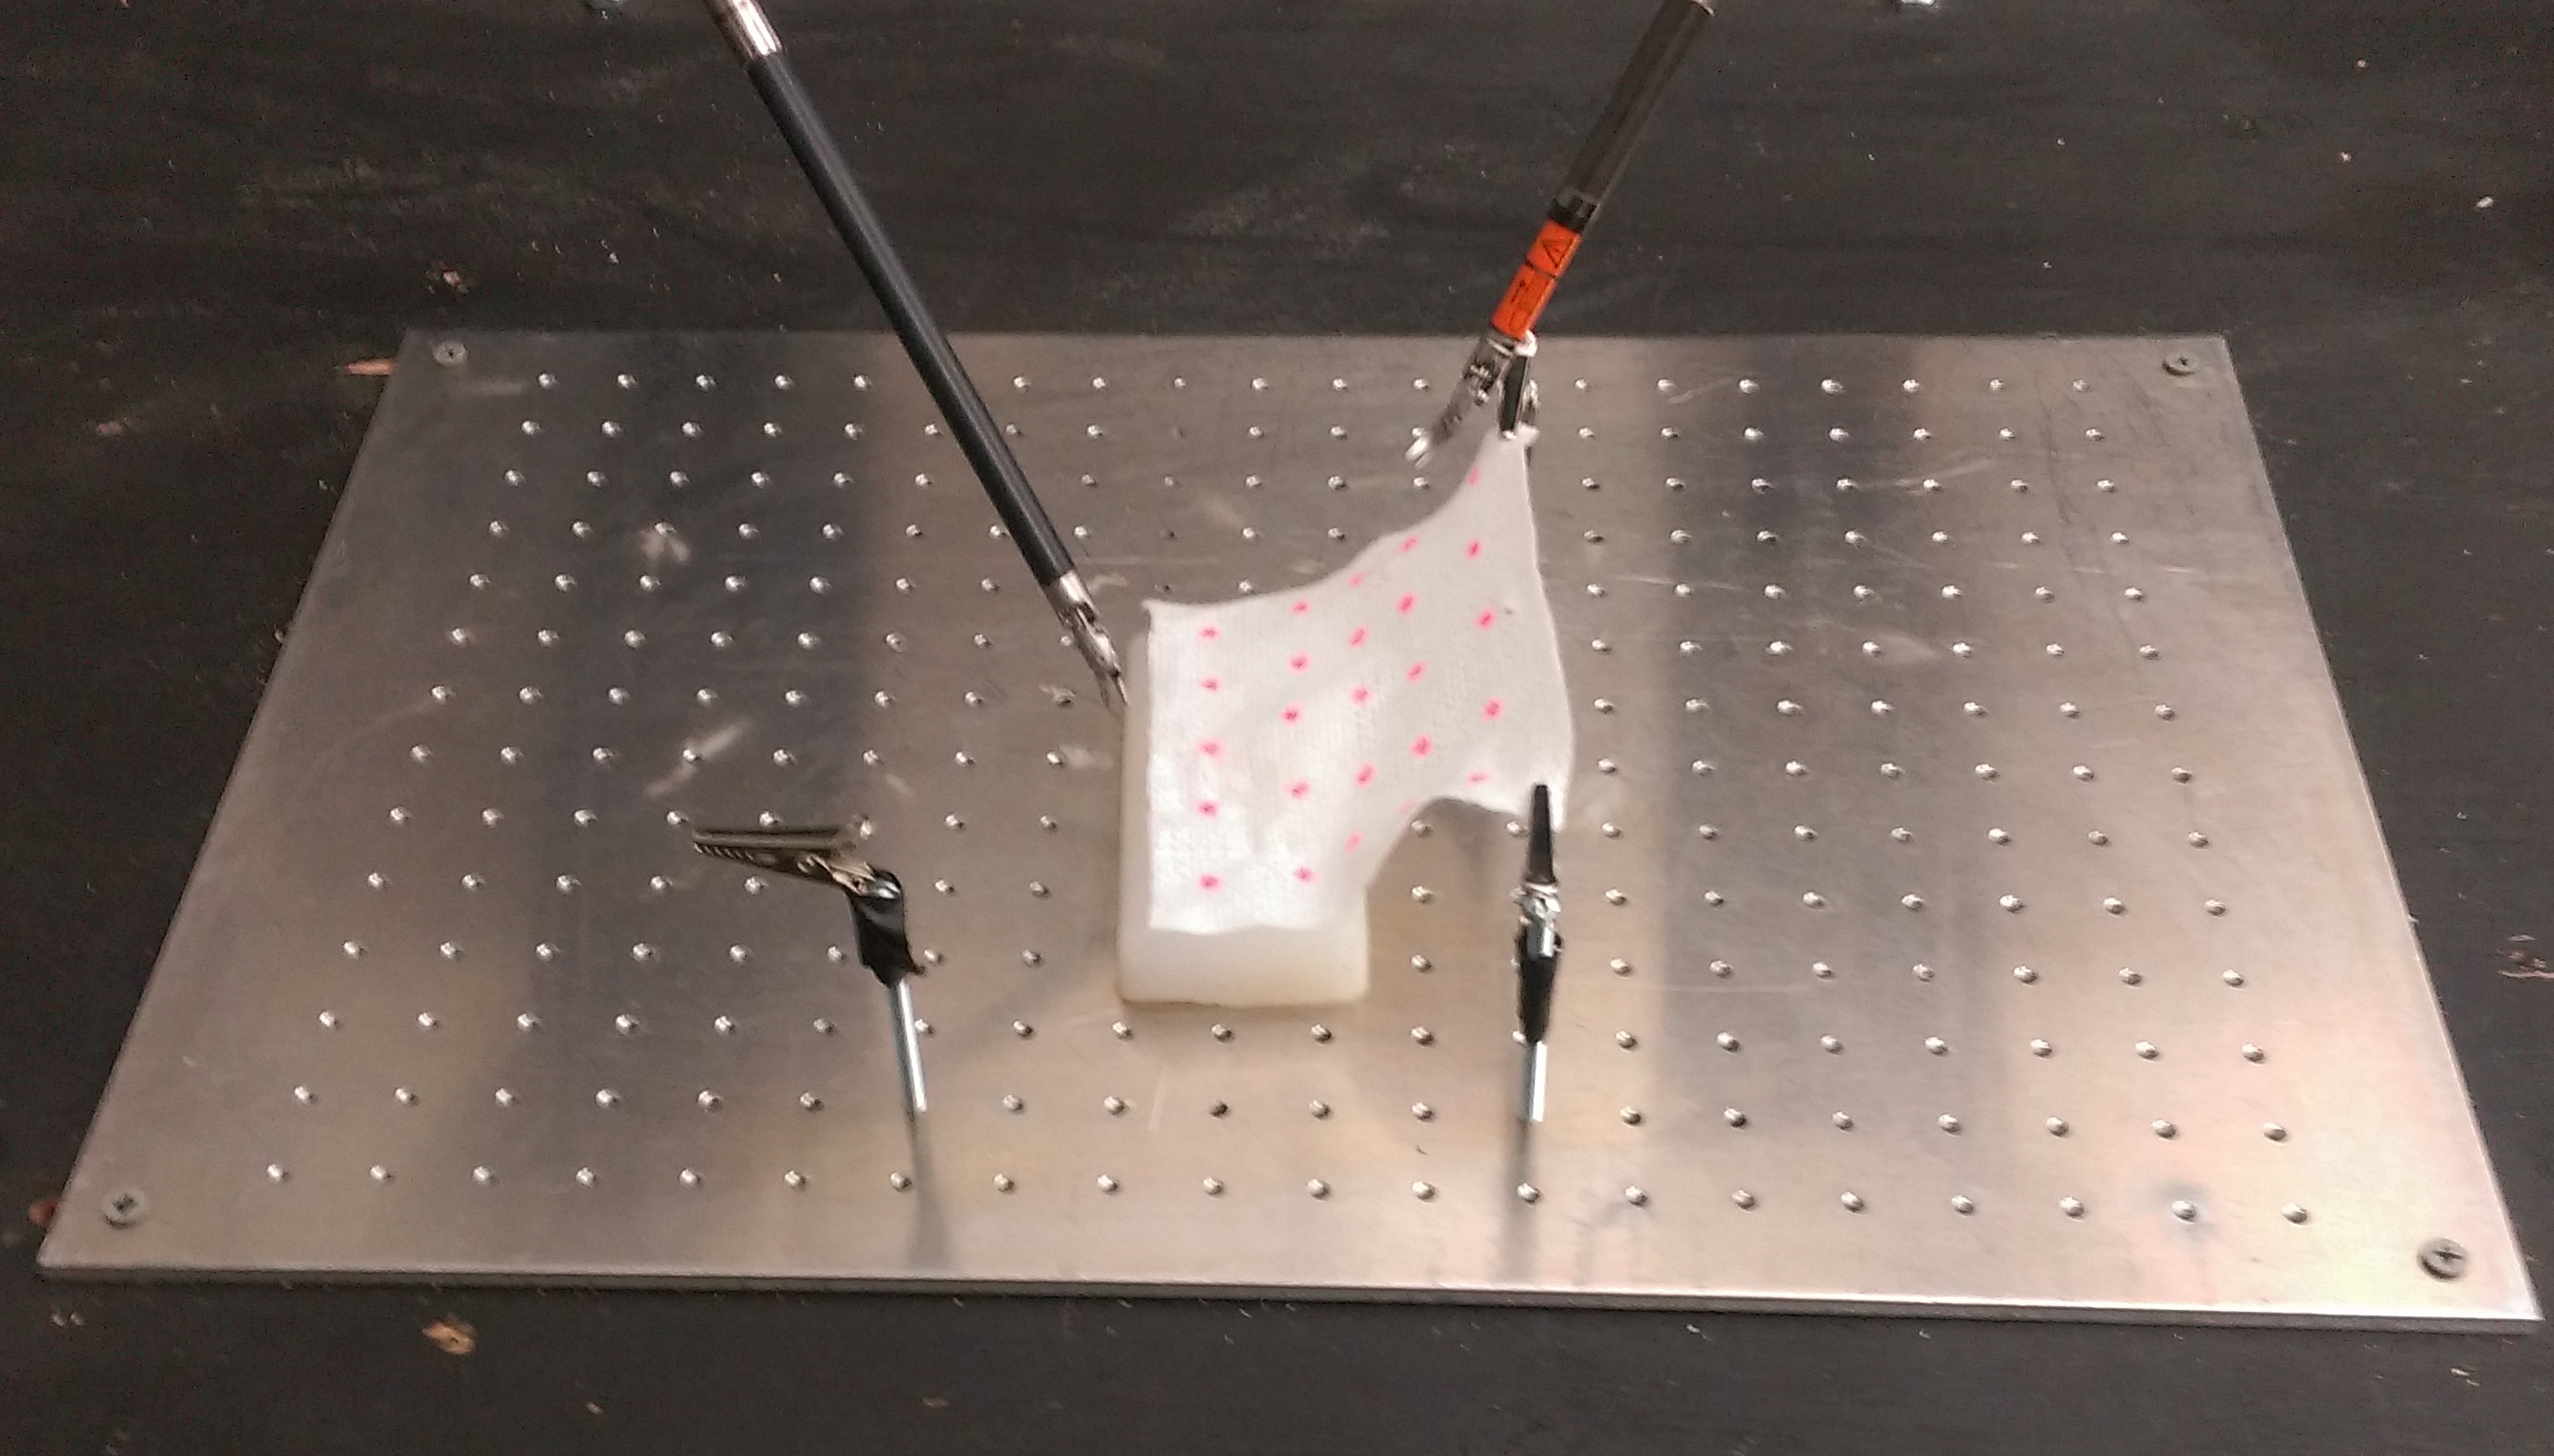
\includegraphics[width=0.8\columnwidth]{exp/IMAG0249.jpg}
    \caption{A sheet of surgical gauze is fixtured at the two far corners using a pair of clips. The unclipped part of the gauze is allowed to rest on soft silicone padding. The robot's task is to reach for the unclipped part, grasp it, lift the gauze, and tension the sheet to be as planar as possible.
An open-loop policy typically fails on this task because it requires some feedback of whether gauze is properly grasped, how the gauze has deformed after grasping, and visual feedback of whether the gauze is planar.The fiducial markers used to track the gauze are seen in red.
    }
    \label{exp:dvrk2}
% \vspace{-15pt}
\end{figure}


\subsection{Physical Experiments with the da Vinci Surgical Robot}
In the next set of experiments, we evaluate \hirl on two tasks on the da Vinci Surgical Robot.
The da Vinci Research Kit is a surgical robot originally designed for tele-operation, and we consider autonomous execution of surgical subtasks.
Based on a chessboard calibration, we found that the robot has an RMSE kinematic error of 3.5 mm, and thus, requires feedback from vision for accurate manipulation. 
In our robotic setup, there is an overhead endoscopic stereo camera that can be used to find visual features for learning, and it is located 650mm above the workspace.
This camera is registered to the workspace with a RSME calibration error of 2.2 mm.

\begin{figure*}[t]
\centering
    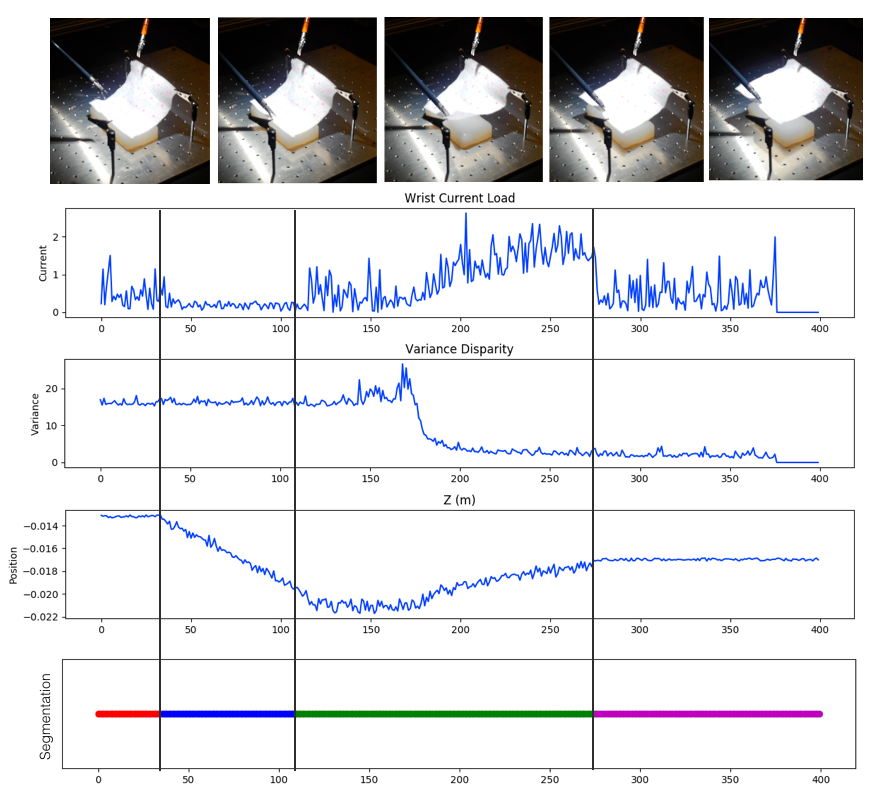
\includegraphics[width=0.8\textwidth]{exp/signals2.png}
    \caption{A representative demonstration of the deformable sheet tensioning task with relevant features plotted over time. \hirl identifies 4 segments which correspond to reaching, grasping, lifting, and tensioning. 
    }
    \label{exp:dvrk3}
% \vspace{-15pt}
\end{figure*}


\subsubsection{Deformable Sheet Tensioning: } In the first experiment, we consider the task of deformable sheet tensioning. The experimental setup is pictured in Figure \ref{exp:dvrk2}. A sheet of surgical gauze is fixtured at the two far corners using a pair of clips. The unclipped part of the gauze is allowed to rest on soft silicone padding. The robot's task is to reach for the unclipped part, grasp it, lift the gauze, and tension the sheet to be as planar as possible.
An open-loop policy typically fails on this task because it requires some feedback of whether gauze is properly grasped, how the gauze has deformed after grasping, and visual feedback of whether the gauze is planar.
The task is sequential as some grasps pick up more or less of the material and the flattening procedure has to be accordingly modified.

The state-space is the 6 DoF end-effector position of the robot, the current load on the wrist of the robot, and a visual feature measuring the flatness of the gauze.
This is done by a set of fiducial markers on the gauze which are segmented by color using the stereo camera.
Then, we correspond the segmented contours and estimate a $z$ position for each marker (relative to the horizontal plane).
The variance in the $z$ position is a proxy for flatness and we include this as a feature for learning (we call this disparity).
The action space is discretized into an 8 dimensional vector ($\pm x$, $\pm y$, $\pm z$, open/close gripper) where the robot moves in 2mm increments.

We provided 15 demonstrations through a keyboard-based tele-operation interface.
The average length of the demonstrations was 48.4 actions (although we sampled observations at a higher frequency about 10 observations for every action).
From these 15 demonstrations, \hirl identifies four segments. Figure \ref{exp:dvrk3} illustrates the segmentation of a representative demonstration with important states plotted over time.
One of the segments corresponds to moving to the correct grasping position, one corresponds to making the grasp, one lifting the gauze up again, and one corresponds to straightening the gauze.
One of the interesting aspects of this task is that the segmentation requires multiple features.
Figure \ref{exp:dvrk3} plots three signals (current load, disparity, and z position), and segmenting any single signal may miss an important feature. 

Then, we tried to learn a policy from the rewards constructed by \hirl.
In this experiment, we initialized the policy learning phase of \hirl with the Behavioral Cloning policy.
We define a Q-Network with a single-layer Multi-Layer Perceptron with 32 hidden units and sigmoid activation.
For each of the segments, we apply Behavioral Cloning locally with the same architecture as the Q-network (with an additional softmax over the output layer) to get an initial policy. We rollout 100 trials with an $\epsilon=0.1$ greedy version of these segmented policies.


The learning results of this experiment are summarized below with different baselines.
The value of the policy is a measure of average disparity over the gauze accumulated over the task (if the gauze is flatter longer, then the value is greater).
As a baseline, we applied RL for 100 rollouts with no other information. RL did not successfully grasp the gauze even once.
Next, we applied behavioral cloning (BC) directly.
BC was able to reach the gauze and but not successfully grasping it.
Then, we applied the segmentation from \hirl  and applied BC directly to each local segment (without further refinement). 
This was able complete the full task with a cumulative disparity score of $-3516$.
Finally, we applied all of \hirl and found the highest-value results ($-2241$ 36\% relative improvement).
For comparison, we applied \hirl without the BC initialization and found that it was only successful at the first two steps.
This indicates that in real tasks the initialization is crucial.

% Please add the following required packages to your document preamble:
% \usepackage[table,xcdraw]{xcolor}
% If you use beamer only pass "xcolor=table" option, i.e. \documentclass[xcolor=table]{beamer}
\begin{table}[ht]
\centering
\scriptsize
\caption{Results from the deformable sheet tensioning experiment}
\label{my-label}
\begin{tabular}{llll}
\rowcolor[HTML]{000000} 
{\color[HTML]{FFFFFF} Technique} & {\color[HTML]{FFFFFF} \# Demonstrations} & {\color[HTML]{FFFFFF} \# Rollouts} & {\color[HTML]{FFFFFF} Value} \\
RL (ab initio)                   & -                                        & 100                                & -8210                        \\
BC                               & 15                                       & -                                  & -7591                        \\
Segmentation+BC                  & 15                                       & -                                  & -3516                        \\
SWIRL+MF (no init)                  & 15                                       & 100                                & -6128                        \\
SWIRL+IRL (no init)                  & 15                                       & 100                                & -5798                        \\
\textbf{SWIRL+MF (BC init)}                  & 15                                       & 100                                & \textbf{-3110}     \\
\textbf{SWIRL+IRL (BC init)}                  & 15                                       & 100                                & \textbf{-2241}                       
\end{tabular}
\end{table}


\subsubsection{Surgical Line Cutting: }
In the next experiment, we evaluate generalization to different task instances.
We apply \hirl to learn to cut along a marked line in gauze similar to ~\cite{murali2015learning}.
This is a multi-step problem where the robot starts from a random initial state, has to move to a position that allows it to start the cut, and then cut along the marked line.
We provide the robot 5 kinesthetic demonstrations by positioning the end-effector and then following various marked straight lines.
The state-space of the robot included the end-effector position $(x,y)$ as well as a visual feature indicating its pixel distance to the marked line $(pix)$.
This visual feature is constructed using OpenCV thresholding for the black line.
Since the gauze is planar, the robot's actions are unit steps in the $\pm x, \pm y$ axes.
Figure\,\ref{exp:dvrk1} illustrates the training and test scenarios.

\hirl identifies two segments corresponding to the positioning step and the termination.
The learned reward function for the position step minimizes $x,y,pix$ distance to the starting point and for the cutting step the reward function is more heavily weighted to minimize the $pix$ distance.
We defined task success as positioning within $1$\,cm of the starting position of the line and during the following stage, missing the line by no more than $1$\,cm (estimated from pixel distance).
We evaluated the model-free version of \hirl, Q-Learning, and Behavioral Cloning with an SVM.
\hirl was the only technique able to achieve the combined task.

We evaluated the learned tracking policy to cut gauze.
We ran trials on different sequences of curves and straight lines. 
Out of the 15 trials, 11 were successful.
2 failed due to \hirl errors (tracking or position was imprecise) and 2 failed due to cutting errors (gauze deformed causing the task to fail).
1 of the failures was on the 4.5 cm curvature line and 3 were one the 3.5 cm curvature line.

% \begin{figure}[t]
% \centering
%  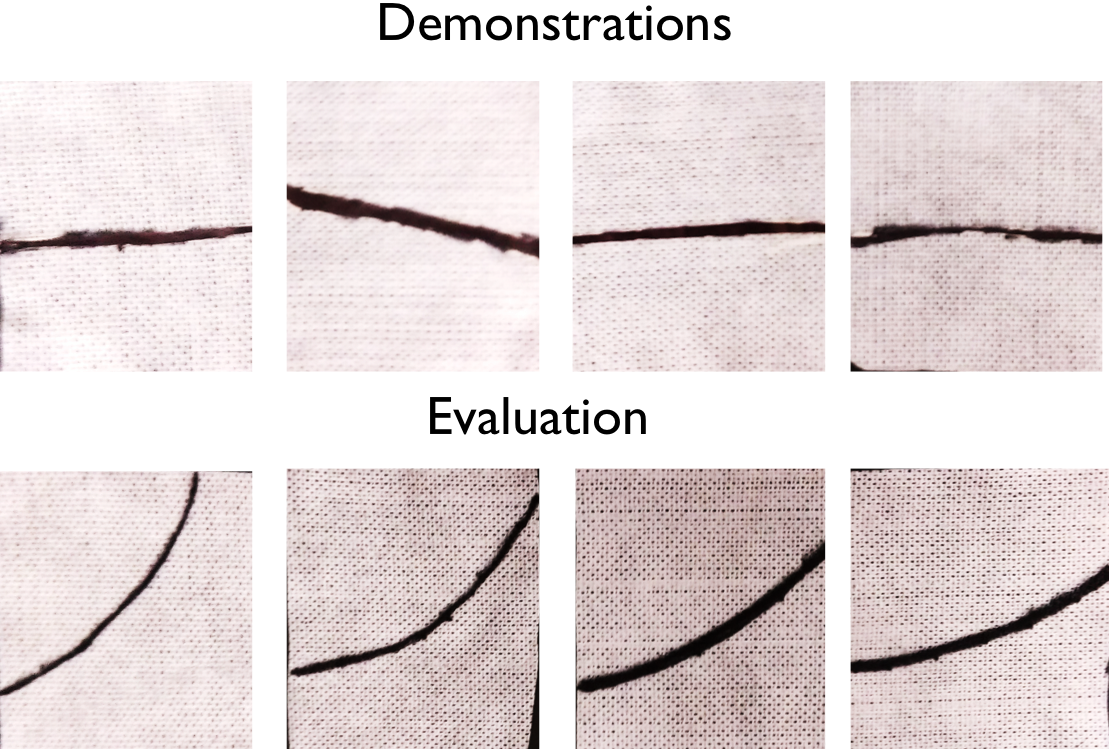
\includegraphics[width=0.7\textwidth]{exp/dvrk-demos-1.png}
%  \caption{We collected demonstrations on the da Vinci surgical robot kinesthetically. The task was to cut a marked line on gauze. We demonstrated the location of the line without actually cutting it. The goal is to infer that the demonstrator's reward function has two steps: position at a start position before the line, and then following the line. We applied this same reward to lines that were not straight nor started in exactly the same position.\label{exp:dvrk1}}
% \end{figure}

% \begin{SCfigure}[10][t]
%     \centering
%     \vspace{-0.5em}
%     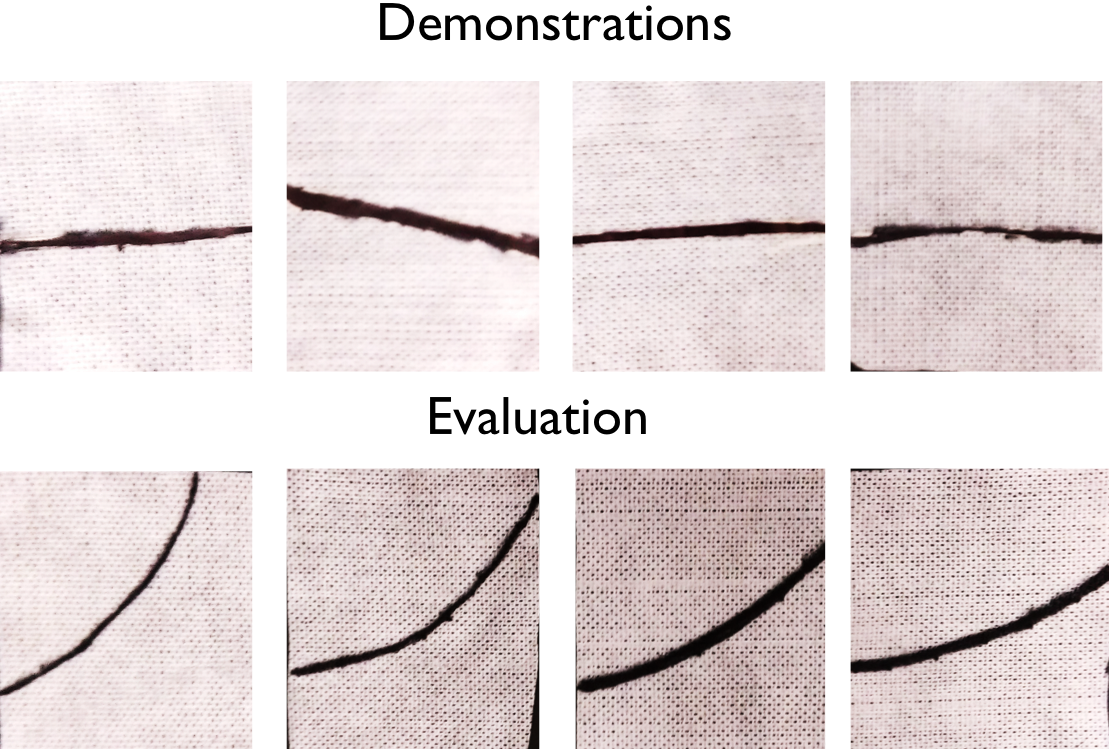
\includegraphics[width=0.5\textwidth]{exp/dvrk-demos-1.png}
%     \caption{We collected demonstrations on the da Vinci surgical robot kinesthetically. The task was to cut a marked line on gauze. We demonstrated the location of the line without actually cutting it. The goal is to infer that the demonstrator's reward function has two steps: position at a start position before the line, and then following the line. We applied this same reward to lines that were not straight nor started in exactly the same position.}
%     \label{exp:dvrk1}
%     \vspace{-1.5em}
% \end{SCfigure}


\begin{figure}[t]
\centering
    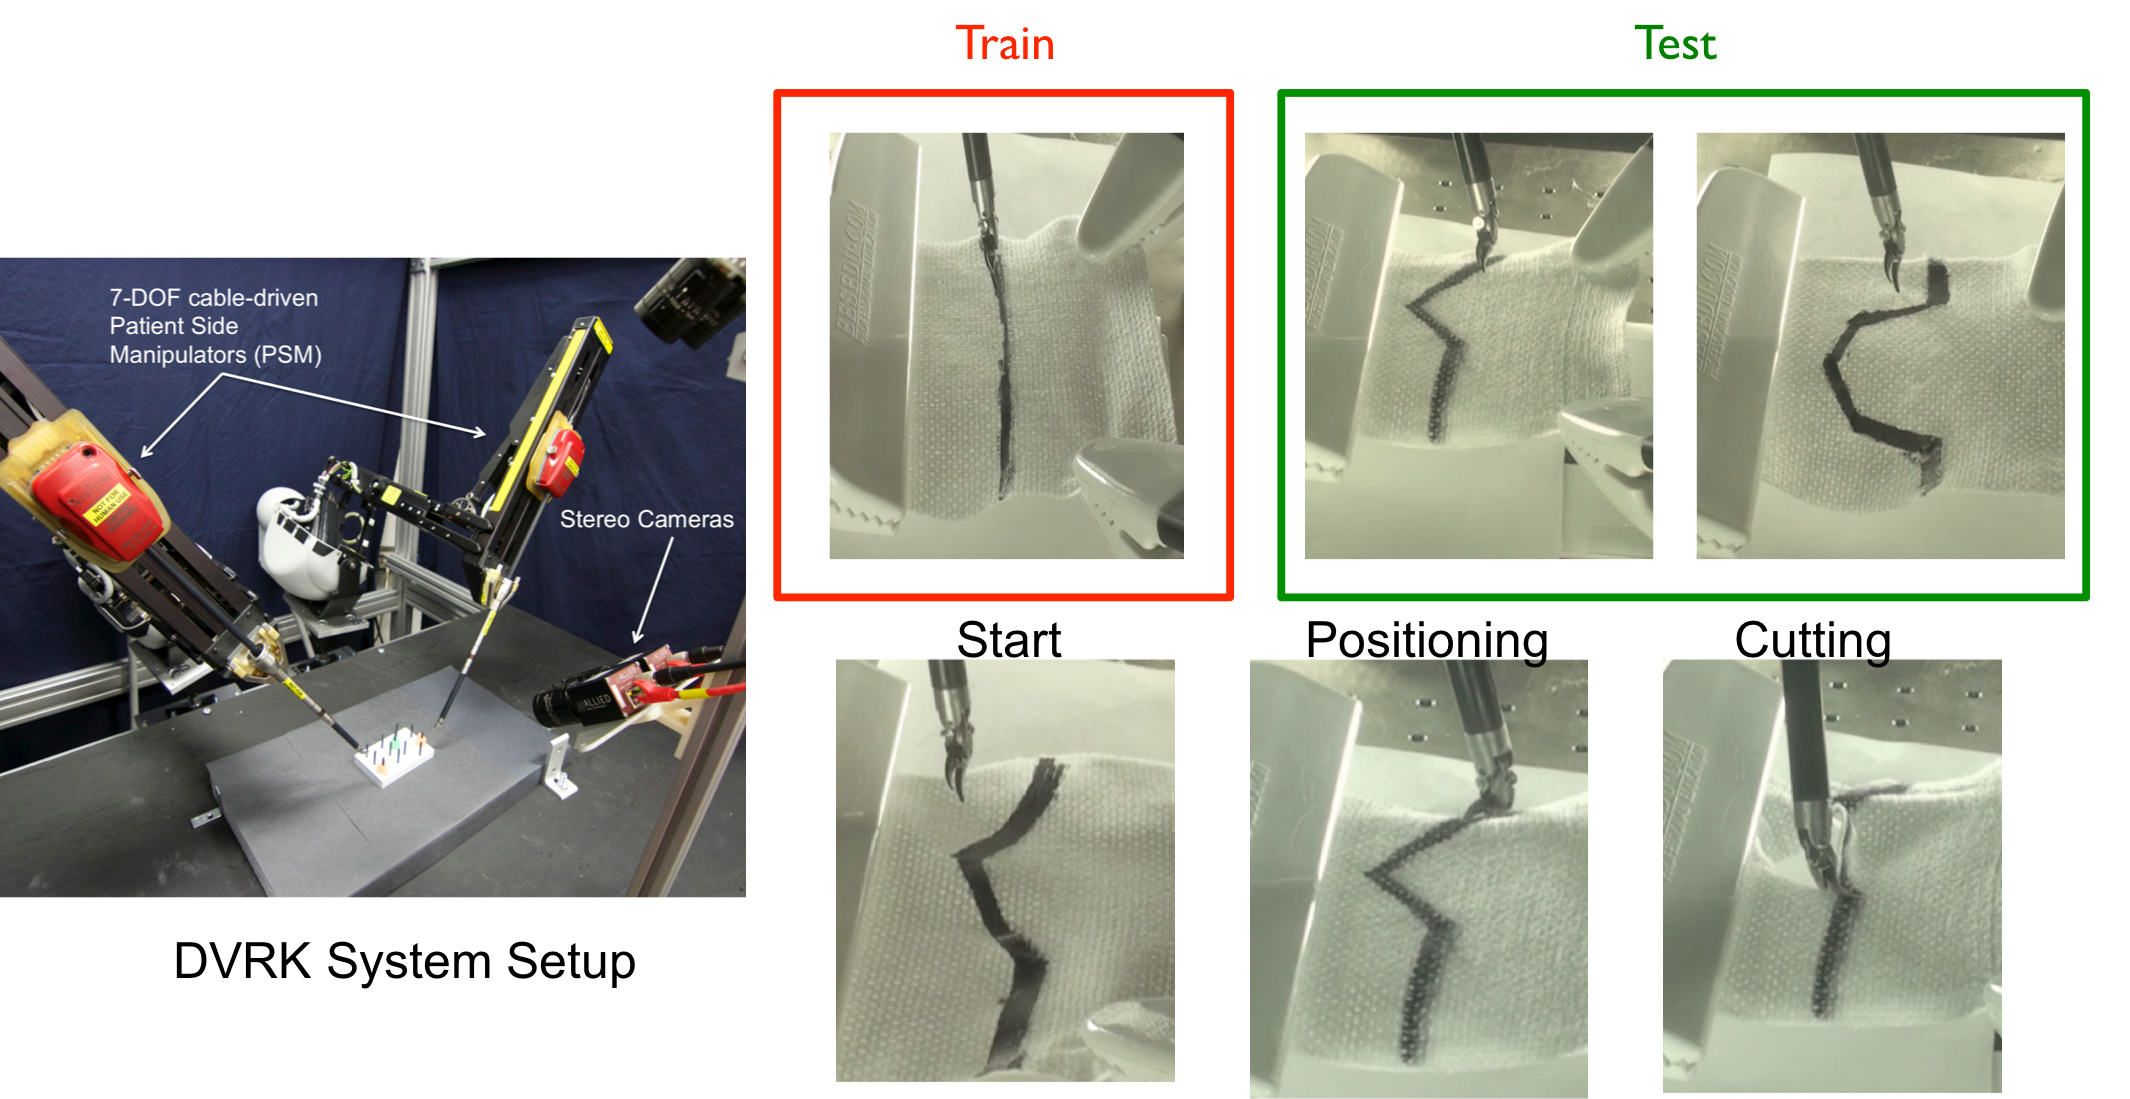
\includegraphics[width=\columnwidth]{exp/dvrk-demo-2.png}
    \caption{
      We collected demonstrations on the da Vinci surgical robot kinesthetically. The task was to cut a marked line on gauze. We demonstrated the location of the line without actually cutting it. The goal is to infer that the demonstrator's reward function has two steps: position at a start position before the line, and then following the line. We applied this same reward to curved lines that started in different positions.
    }
    \label{exp:dvrk1}
% \vspace{-15pt}
\end{figure}

\begin{table*}[ht]
    \centering
    \caption{With 5 kinesthetic demonstrations of following marked straight lines on gauze, we applied \hirl to learn to follow lines of various curvature. After 25 episodes of exploration, we evaluated the policies on the ability to position in the correct cutting location and track the line. We compare to SVM on each individual segment. SVM is comparably accurate on the straight line (training set) but does not generalize well to the curved lines.
    \label{dvrk:res1}}
    \resizebox{\linewidth}{!}{% put in textwidth
    \begin{tabular}{c||c|c|c|c}
    \hline
    \rowcolor[HTML]{CBCEFB} 
    Curvature Radius (cm) & SVM Pos. Error (cm) & SVM Tracking Error (cm) & \hirl Pos. Error (cm) & \hirl Tracking Error (cm) \\
     \hline \hline
    straight & 0.46 & 0.23 & 0.42 & 0.21  \\
    \rowcolor[HTML]{E0E0E0} 
    4.0 & 0.43 & 0.59 & 0.45 & 0.33 \\
    3.5 & 0.51 & 1.21 & 0.56 & 0.38 \\
    \rowcolor[HTML]{E0E0E0} 
    3.0 & 0.86 & 3.03 & 0.66 & 0.57 \\
    2.5 & 1.43 & {\color{red}-} & 0.74 & 0.87 \\
    \rowcolor[HTML]{E0E0E0} 
    2.0 & - & - & 0.87 & 1.45 \\
    1.5 & - & - & 1.12 & 2.44 \\
     \hline
    \end{tabular}
    }
    % \vspace{-10pt}
\end{table*}

Next, we characterized the repeatability of the learned policy.
We applied \hirl to lines of various curvature spanning from straight lines to a curvature radius of 1.5 cm.
Table \ref{dvrk:res1} summarizes the results on lines of various curvature.
While the SVM approach did not work on the combined task, we evaluated its accuracy on each individual step to illustrate the benefits of \hirl.
On following straight lines, SVM was comparable to \hirl in terms of accuracy.
However, as the lines become increasingly curved, \hirl generalizes more robustly than the SVM.
A single SVM has to learn both the positioning and cutting policies. The combined policy is much more complicated than the individual policies, e.g., go to a  goal and follow a line.


